\section*{Aufgabe 1}

Es soll mithilfe des Metropolis-Algorithmus ein einzelner Spin \(\sigma = \pm 1\) mit der Energie \(E = -\sigma H\) im äußeren Magnetfeld \(H\) simuliert werden.
Die Vorschlagswarscheinlichkeit für einen Spin-Flip \(\sigma \rightarrow -\sigma\) ist dabei \(V_{\uparrow \downarrow} = V_{\downarrow \uparrow} = 1\). Die Akzeptanzwahrscheinlichkeit ergibt sich aus
\begin{equation*}
  A_{\uparrow \downarrow} = \min{\left(1, \frac{P_\downarrow}{P_\uparrow} \right)}.
\end{equation*}
Mit \(k_\text{B}T = 1\) wird numerisch die Magnetisierung
\begin{equation*}
  \langle m \rangle = \frac{1}{N} \sum_{k=0}^N m_{i_\text{N}}
\end{equation*}
bestimmt, wobei \(N\) die Anzahl der Schritte des Metropolis-Algorithmus ist.
Dies wird für \(\num{1e4}\) Werte von \(H \in [-5,5]\) mit jeweils \(\num{1e5}\) Schritten durchgeführt und anschließend mit dem analytischen Ergebnis
\begin{equation*}
  m_\text{analytisch} = \tanh{\!(H)}
\end{equation*}
verglichen.
In Abbildung \ref{fig:vergleich} sind die numerischen und analytischen Werte für die Magnetisierung aufgetragen. Dabei ist zu sehen, dass die beiden Verläufe genau aufeinander liegen.
\begin{figure}
  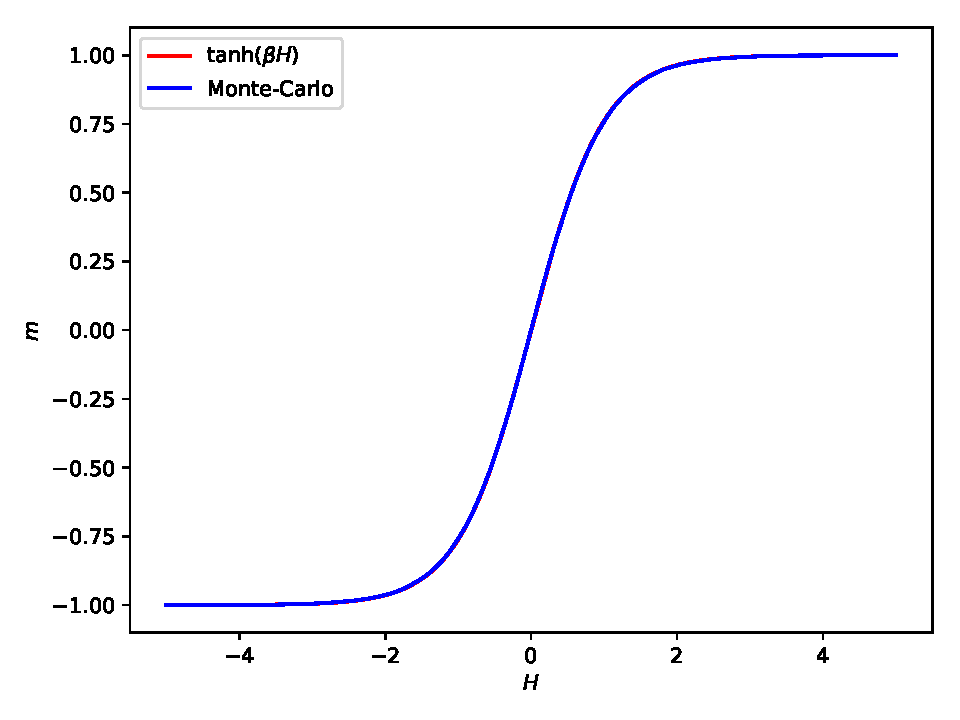
\includegraphics[width=0.8\textwidth]{A1/build/vergleich.pdf}
  \caption{Vergleich der analytischen und numerischen Magnetisierung.}
  \label{fig:vergleich}
\end{figure}
Da mit dem bloßen Auge keine Abweichungen zu erkennen sind, ist in Abbildung \ref{fig:differenz} die relative Differenz
\begin{equation*}
  \frac{m_\text{analytisch} - m_\text{MC}}{m_\text{MC}}
\end{equation*}
aufgetragen.
\begin{figure}
  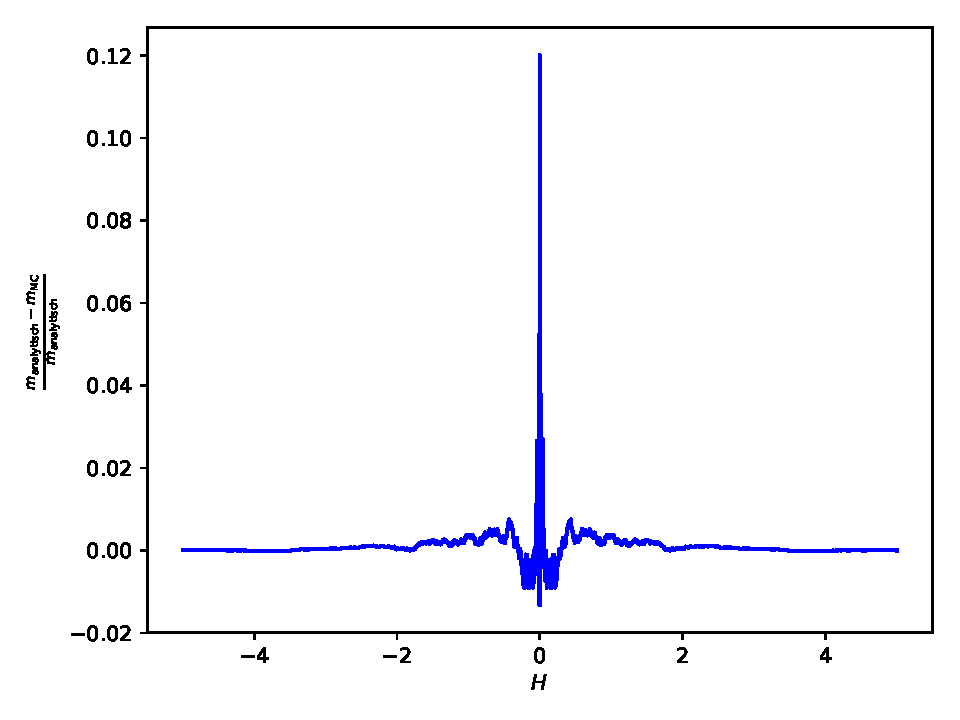
\includegraphics[width=0.8\textwidth]{A1/build/rel_differenz.pdf}
  \caption{Relative Differenz von \(m_\text{analytisch}\) und \(m_\text{MC}\) bei einem Seed von \(2\).}
  \label{fig:differenz}
\end{figure}
Hier ist zu sehen, dass tatsächlich Abweichungen vorliegen. Diese betragen aber im Wesentlichen weniger als \(\SI{2}{\%}\) und sind damit vernachlässigbar klein.
Nur bei \(H=0\) ergibt sich eine größere Abweichung, da es statistisch sehr unwahrscheinlich ist, dass sich die Spins exakt wegheben.
Der Verlauf der Abweichungen variiert natürlich je nachdem welcher Seed gewählt wird, die absoluten Größenordnungen bleiben aber ungefähr gleich.
